\documentclass{article}

\usepackage[a4paper, top=2cm, bottom=3cm]{geometry}
\usepackage[ngerman]{babel}
\usepackage{csquotes}

\usepackage{booktabs}
\usepackage{mathtools}
\usepackage{amssymb}
\usepackage{enumitem}
\usepackage{amsmath}
\usepackage{hyperref}

\usepackage{siunitx}
\usepackage[version=4]{mhchem}

\usepackage{biblatex}
\DefineBibliographyStrings{ngerman}{
  urlseen = {Abruf vom}
}
\addbibresource{quellen.bib}

\newcommand{\proofeq}{\overset{!}{=}}
\newcommand{\proofeqv}{\overset{!}{\Leftrightarrow}}
\newcommand{\equivalent}{\overset{\scriptscriptstyle\wedge}{=}}
\DeclarePairedDelimiter\ceil{\lceil}{\rceil}
\DeclarePairedDelimiter\floor{\lfloor}{\rfloor}

\date{7.03.2022}
\title{Physikalisches Grundpraktikum Teil I \\ (Mechanik und Thermodynamik) \\ Versuch 5 Lufballon mit \ce{CO2}}
\author{Wafaa Al Nachawti, Finn Wagner}

\begin{document}
    \maketitle

    \section{Versuchsziel und Versuchsmethode}
    In diesem Versuch wird die Dichte von \ce{CO2} über die Fallzeit eines mit \ce{CO2} gefüllten Luftballons bestimmt.
    Der Fall des Luftballons wird als Bewegung eines kugelförmigen Körpers in einer Flüssigkeit (Luft oder Luft als Quasi-Flüssigkeit) mit laminarer Strömung approximiert.

    \section{Grundlagen}
    Wir füllen zwei Luftballons, einmal mit Luft und einmal mit \ce{CO2}. Auf beide Luftballons wirkt die gleiche Auftriebskraft, da sie das gleiche Volumen an Luft verdrängen.
    Aber, da sich ihre Massen unterscheiden wirkt auf den mit \ce{CO2} gefüllten Luftballon, wie wir später sehen werden, auf Grund der höheren Dichte von \ce{CO2}
    eine stärkere Gewichtskraft, die mehr von der Geschwindigkeits abhängigen Reibungskraft überwinden kann. Der mit \ce{CO2} gefüllte Luftballon fällt schneller.
    Aus dieser Beziehung zwischen Dichte und Geschwindigkeit stellen wir eine Formel auf und können durch Messen des Volumens der Luftballons, sowie der Fallgeschwindigkeiten
    zunächst den Faktor zwischen den beiden Dichten, aber da wir die Dichte von Luft bereits kennen\cite{Aufgabenstellung}, die Dichte von \ce{CO2} berechnen.

    TODO: Co2 aus Wasser lösen, Druck Gleichgewicht etc.

    \section{Formeln}
    Auf jeden Körper wirkt im Schwerefeld der Erde eine Zentralkraft Richtung Erdmittelpunkt, proportional zur Masse des Körpers.
    \begin{equation} \label{eq:schwerkraft}
        F_G = m \cdot g    
    \end{equation}
    Die Masse eines Körpers (mit Dichte \(\rho_K\)) können wir auch über seine Dichte und sein Volumen ausdrücken mit der Beziehung:
    \begin{equation} \label{eq:masse_dichte_rel}
        m = \rho_K \cdot V \cdot g
    \end{equation}
    Weiterhin wirkt auf Körper mit echter Ausdehnung (keine Punktmasse) in Flüssigkeiten/Gasen wie Luft eine Auftriebskraft, 
    die durch Verdrengung des Mediums entsteht. Sie ist abhängig vom verdrengten Volumen und der Dichte des Mediums (Gases \(\rho_G\)) in dem sich der Körper befindet.
    \begin{equation} \label{eq:auftrieb}
        F_A = \rho_{G} \cdot V \cdot g
    \end{equation}
    Als dritte Kraft wirkt bei unserem Versuch eine Reibungskraft gegen den Fall des Luftballons an.
    Die Stokes'sche Reibung ist proportional zur Geschwindigkeit \(v\), dem Radius \(r\) des Luftballons, so wie der Viskosität \( \eta \) der Luft.
    \begin{equation} \label{eq:stokes_reibung}
        F_R = 6 \pi \cdot r \cdot \eta \cdot v
    \end{equation}
    TODO: Wir setzen hier Stokes'sche Reibung an, da wir uns vollständig im Bereich laminarer Strömung aufgrund sehr kleiner Geschwindigkeiten befinden
    Der Luftballon wird als von der Schwerkraft nach unten beschleunigt, vom Auftrieb und von der Reibungskraft gebremst.
    Der Luftballon beschleunigt bis zu seiner maximalen Fallgeschwindigkeit\cite{Fall-Luftwiederstand} und fällt ab dann mit einer konstanten Geschwindigkeit weiter,
    wird also nicht mehr weiter beschleunigt, da auf den Ballon keine resultierende Kraft mehr wirkt\ref{eq:gleichgewicht}.
    Da für unsere Gegebenheiten (TODO: machen in Fehlerrechnung) die Zeit in der der Luftballon beschleunigt im Vergleich zur gesamten Fallzeit sehr gering ist,
    setzen wir für den gesamten Fall das Kräftegleichgewicht an:
    \begin{equation} \label{eq:gleichgewicht}
        F_G = F_A + F_R
    \end{equation}
    Wir approximieren also, das der Luftballon auf der gesamten Strecke \(h\) mit der selben Geschwindigkeit \(v\) fällt. Er braucht dazu die Zeit \(t_{Fall}\)
    \begin{equation} \label{eq:geschwindigkeit}
        v = \frac{h}{t_{Fall}}
    \end{equation}
    Die Endgeschwindigkeit des Ballons lässt sich aus dem Kräftegleichgewicht\ref{eq:gleichgewicht} durch einsetzen der Stokes'schen Reibung ausdrücken:
    \begin{equation}
        \begin{gathered} \label{eq:stokes_geschwindigkeit}
            F_G = F_A + F_R \Rightarrow F_R = F_G - F_A \\
            \Rightarrow 6 \pi \cdot r \cdot \eta \cdot v = F_G - F_A \\
            \Rightarrow v = \frac{ F_G - F_A }{ 6 \pi \cdot r \cdot \eta }
        \end{gathered}
    \end{equation}
    Wir setzen nun Gleichung\ref{eq:geschwindigkeit} und Gleichung\ref{eq:stokes_geschwindigkeit} gleich.
    \begin{equation} \label{eq:fall_halb}
        \frac{h}{t_{Fall}} = \frac{ F_G - F_A }{ 6 \pi \cdot r \cdot \eta }
    \end{equation}
    Im Experiment werden zwei Luftballons, einer gefüllt mit \ce{CO2} und einer gefüllt mit Luft, aus der selben Höhe \(h\) fallengelassen.
    Die Masse m eines solchen gefüllten Luftballons setzt sich aus der Masses \( m_h \) des Ballons (der Ballonhülle aus Gummi), sowie dem in ihm enthaltenen Gas\ref{eq:masse_dichte_rel} zusammen
    Wir setzen diese Masse in die Formel für die Schwerkraft\ref{eq:schwerkraft} ein:
    \begin{equation} \label{eq:schwerkraft_ballon}
        F_G = m \cdot g = m_H \cdot g + \rho \cdot V \cdot g = \left( m_H + \rho \cdot V \right) \cdot g
    \end{equation}
    Die Schwerkraft\ref{eq:schwerkraft_ballon}, sowie die Auftriebskraft\ref{eq:auftrieb} setzen wir in die Gleichung\ref{eq:fall_halb} ein:
    \begin{equation} \label{eq:fall}
        \frac{h}{t_{Fall}} = \frac{ \left( m_H + \rho_{F\ddot{u}llung} \cdot V \right) \cdot g - \rho_{Medium} \cdot V \cdot g }{ 6 \pi \cdot r \cdot \eta_{Medium} }
    \end{equation}
    Zu unterscheiden sind die beiden Dichten. \(\rho_{F\ddot{u}llung}\) ist die Dichte des Gases im Luftballon, \(rho_{Medium}\) die Dichte des Gases in der Atmosphäre.
    Für den Luftballon gefüllt mit Luft wird die Formel\ref{eq:fall} zu:
    \begin{equation} \label{eq:fall_luft}
        \frac{h}{t_{Luft}} = \frac{ \left( m_H + \rho_{Luft} \cdot V \right) \cdot g - \rho_{Luft} \cdot V \cdot g }{ 6 \pi \cdot r \cdot \eta_{Luft} }
    \end{equation}
    Und für den Luftballon gefüllt mit \ce{CO2} wird die Formel\ref{eq:fall} zu:
    \begin{equation} \label{eq:fall_co2}
        \frac{h}{t_{\ce{CO2}}} = \frac{ \left( m_H + \rho_{\ce{CO2}} \cdot V \right) \cdot g - \rho_{Luft} \cdot V \cdot g }{ 6 \pi \cdot r \cdot \eta_{Luft} }
    \end{equation}
    Wir teilen nun die Formel für den Fall in \ce{CO2}\ref{eq:fall_co2} durch die für den Fall in Luft\ref{eq:fall_luft} und vereinfachen:
    % TODO: \cancel{} für alles was noch sinnvoll weggestrichen
    \begin{equation} \label{eq:calc_rho_faktor}
        \begin{gathered}
            \frac{ \frac{h}{t_{\ce{CO2}}} }{ \frac{h}{t_{Luft}} } = \frac{ t_{Luft} }{ t_{\ce{CO2}} } =
            \frac{ \frac{ \left( m_H + \rho_{\ce{CO2}} \cdot V \right) \cdot g - \rho_{Luft} \cdot V \cdot g }{ 6 \pi \cdot r \cdot \eta_{Luft} } }
                 { \frac{ \left( m_H + \rho_{Luft} \cdot V \right) \cdot g - \rho_{Luft} \cdot V \cdot g }{ 6 \pi \cdot r \cdot \eta_{Luft} } } = \\
            \frac{ \left( m_H + \rho_{\ce{CO2}} \cdot V \right) \cdot g - \rho_{Luft} \cdot V \cdot g }{ \left( m_H + \rho_{Luft} \cdot V \right) \cdot g - \rho_{Luft} \cdot V \cdot g } =
            \frac{ \left( m_H + \rho_{\ce{CO2}} \cdot V \right) \cdot g - \rho_{Luft} \cdot V \cdot g }{ m_H \cdot g + \left( \rho_{Luft} \cdot V \cdot g - \rho_{Luft} \cdot V \cdot g \right) } = \\
            \frac{ \left( m_H + \rho_{\ce{CO2}} \cdot V \right) - \rho_{Luft} \cdot V }{ m_H } = \\
            \frac{ m_H + V \cdot \left( \rho_{\ce{CO2}} - \rho_{Luft} \right)}{ m_H } = 1 + \frac{V}{m_H} \left( \rho_{\ce{CO2}} - \rho_{Luft} \right)
        \end{gathered}
    \end{equation} 
    Gleichung\ref{eq:calc_rho_faktor} formen wir im letzen Schritt noch nach \(\rho_{\ce{CO2}}\) auf:
    \begin{equation} \label{eq:calc_rho_co2}
        \rho_{\ce{CO2}} = \rho_{Luft} + \left( \frac{t_{Luft}}{t_{\ce{CO2}}} - 1 \right) \frac{m_H}{V}
    \end{equation}

    TODO: Luftballon Kugel approximieren. Ein kugelförmiger Körper mit Dichte \(\rho_K\) in einer Flüssigkeit mit Dichte \(\rho_{Fl}\) fällt in eben jener Flüssigkeit nach unten

    \section{Versuchsaufbau}
        \begin{figure}[h]
            \centering
            \begin{minipage}[t]{0.4\textwidth}\label{fig:versuch_schematik}
                \includegraphics[height=6cm]{kräfte.png}
                \caption{Schematische Darstellung des Versuchs und der auftretenden Kräfte}
            \end{minipage}
            \hfill
            \begin{minipage}[t]{0.4\textwidth}\label{fig:abmessungen}
                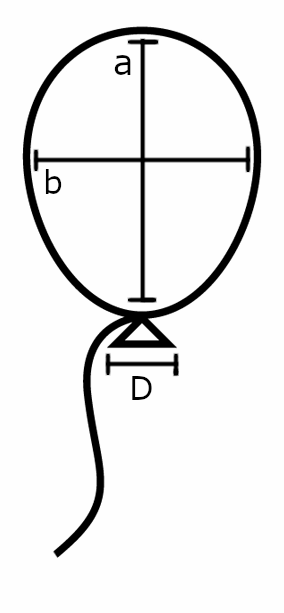
\includegraphics[height=6cm]{luftballons.png}
                \caption{Messgrößen am Luftballon}
            \end{minipage}
        \end{figure} TODO: Allign

        \subsection{Material}
        \begin{itemize}
            \item 2 Luftballons
            \item 1 Flasche Mineralwasser Classic; Wasser mit viel Kohlensäure
            \item Smartphone zum Aufnehmen eines Videos
            \item Maßband mit mindestens Milimetergenauigkeit, am besten ein weiches Rollbandmaß
            \item 1 Stoppuhr oder Computerprogramm zum auswerten der Zeiten im Video
        \end{itemize}

    \section{Durchführung}
        \subsection{Ballon mit \texorpdfstring{\ce{CO2}}{CO2} aufpumpen}
            \begin{enumerate}
                \item Stülpen Sie den Luftballon (d.h.\ das Mundstück des Luftballons) auf den Hals der Mineralwasserflasche (Abb TODO: Bild hinzufügen)
                \item Schütteln Sie die Wasserflasche wiederholt, um die im Wasser gelöste Kohlensäure in \ce{CO2}-Gas umzuwandeln und den Luftballon dadurch auf zublasen.
                Achten Sie darauf das kein Wasser in den Ballon kommt, um die Masse des Ballons nicht zu verändern.
                \item Der Ballon muss am Ende nicht vollständig aufgeblasen sein; etwa \(\SI{15}{cm}\) sind bereits ausreichend.
                \item Halten sie den Ballon zu und nehmen sie ihn vorsichtig von der Flasche, sodass kein \ce{CO2} eintweicht und knoten Sie ihn zu.
            \end{enumerate}
        
        \subsection{Zweiten Ballon füllen}
            \begin{enumerate}[resume]
                \item Bestimmen Sie die Umfänge des mit \ce{CO2} gefüllten Ballons mithilfe des Maßbands.
                Messen Sie den Umfang vom Mundstück bis zum obersten Punkt (Umfang a), sowie die \enquote{Tallie} (Umfang b) (TODO:ref Bild)
                \item Pusten Sie einen zweiten Ballon (mit Luft) auf. Lassen sie in kleinen Schritten Luft aus dem Ballon und messen Sie wiederholt die Umfänge,
                bis die beiden Luftballons ein identisches Volumen haben.
                \item Knoten Sie den Luftballon zu.
                TODO: Gekennzeichnet?
            \end{enumerate}
        
        \subsection{Fallversuch}
            \begin{enumerate}[resume]
                \item Suchen Sie sich einen Ort als Referenzpunkt in gut \(\SI{2}{Metern}\) Höhe (z.B.\ Oberkante eines Schranks, Türrahmen) und messen Sie
                den Abstand \(h\) zum Boden.
                \item Starten Sie ein Video auf ihrem Handy mit Stativ oder lassen Sie sich von einer zweiten Person helfen.
                Nehmen Sie das Video von etwas weiter weg auf und achten Sie darauf das der Start, sowie das Aufkommen auf dem Boden im Video gut zu sehen sind.
                \item Halten Sie die beiden Luftballons in Höhe \(h\) und lassen Sie sie gleichzeitig fallen. TODO: Ref Video
                \item Wiederholen Sie den Fallversuch 3 mal, nehmen Sie also 2 weitere Videos auf.
            \end{enumerate}
            
        \subsection{Videoauswertung}
            \begin{enumerate}
                \item Messen Sie bei allen aufgenommen Videos die Fallzeiten der Luftballons vom Zeitpunkt an dem sie losgelassen wurden, bis sie auf den Boden aufkommen.
                Dies kann durch mitstoppen mit einer Stoppuhr beim anschauen des Videos oder durch direktes auswerten des Videos mit Hilfe eines geigneten Computerprogramms oder Handyapp
            \end{enumerate}
        TODO: Bilder, 1.Ballon auf Flasche, 2.Ballon auf Flasche geschüttelt, 3. Fallversuch

        Bei unserer Durchführung haben wir uns für die Unterkannte eines Türrahmens entschieden. TODO:
    
    \section{Auswertung}
        Es wurde versucht die beiden Luftballons bestmöglich auf das gleiche Volumen zu bringen.
        Wir berechnen aus den Messungen der Umfänge ein Volumen, was wir für beide Luftballons ansetzen.
        Für a:
        \begin{equation}
            a_1 = \SI{0.475}{m}, a_2 = \SI{0.477}{m} \Rightarrow a = \SI{0.476}{m} 
        \end{equation}
        Für b wurde bei beiden Luftballons der selbe Umfang \(b = \SI{0.45}{m} \) gemessen.
        Wir berchnen den Mittelwert aus \(a\) und \(b\), um den Luftballon besser als Kugel approximieren zu können.
        \begin{equation}
            U = \frac{ \SI{0.476}{m} + \SI{0.45}{m} }{2} = \SI{0.463}{m}
        \end{equation}
        Volumen der Luftballons berechnen:
        \begin{equation} \label{eq:volumen}
            V = \frac{4}{3} \pi {\left( \frac{U}{2 \pi} \right) }^3 = \frac{4}{3} \pi \frac{U^3}{8 \pi^3} = \frac{1}{6} \frac{U^3}{\pi^2}
        \end{equation}
        Wir setzen den Umfang \(U\) ein:
        \begin{equation}
            V =  \frac{1}{6} \frac{{(\SI{0.463}{m})}^3}{\pi^2} = \SI{1.676e-3}{m^3}
        \end{equation}
        
        Berechnen Sie aus den drei Messungen die Mittelwerte und setzen sie ein.

        Mit der Dichte \(\rho_{Luft}\) aus der Aufgabenstellug\cite{Aufgabenstellung}
        und dem Mittelwert der aus den Videos bestimmten Fallzeiten berechnen wir mit Formel\ref{eq:calc_rho_co2} die Dichte von \ce{CO2}:
        \begin{equation}
            \rho_{CO_2} = \SI{1.2041}{\frac{kg}{m^3}} + (\frac{t_{Luft}}{t_{CO_2}} - 1)+\frac{m_H}{V}
        \end{equation}
        TODO: Formel für die Dichte von co2 mit Volumenformel eingesetzt?
        TODO: Trennen Formeln und Auswertung?

    \section{Fehlerrechnung}
        Prallaxe von Video???
        Nicht auf gleiche Höhe am Anfang.
        Luftstömungen?
        
        TODO: Fehler Luftballon aufgepustet nicht Umgebungsluft?
        TODO: Fehler Luft im Co2 ballon, alternativ Sodastream?
        TODO: Schwer zu sehen wann Boden berührt
        TODO: Wiegen sie den Luftballon.
        TODO: Fehler Luftballon wiegt 2g
        TODO: (Wasser in Ballon?)
        TODO: Video aufgenommen ausgewertet mit Media Player Classic?App ausgewertet
        TODO: Beachten Vidoe nur mit 30fps aufgenommen Fehlerrechnung
        TODO: Umfangfehlerrechnung aus Versuch 6 klauen. Hier aber mehr auf schwierig Umfänge zu vergleichen eingehen. Volumenfehler
        TODO: Theoriefehler aus Herleitung???

    \section{Fall auf der Venus}
        Wir bestimmen nun, wie lang der Fall des mit \ce{CO2} gefüllten Luftballons auf der Venus dauern würde. Wir nehmen an,
        das die Atmosphäre der Venus zu \( 100\% \) aus \ce{CO2} besteht. Die Schwerkraft auf der Venus beträgt \(g_{Venus} = \SI{8.87}{\frac{m}{s}}\).
        Die Atmosphäre auf der Venus ist mit mehr als \(\SI{400}{\celsius}\) sehr heiß und die Viskosität ist abhängig von der Temperatur.
        Wir nehmen für diese Rechnung an, das es auf der Venus nur Raumtemparatur mit \(T = \SI{20}{\celsius}\) warm ist.
        Die Viskosität von \ce{CO2} ist dann \( \eta_{\ce{CO2}} = \SI{14.73e-6}{\pascal\cdot\second} \)

        Wir gehen hier beim aufstellen der Formel ähnlich vor wie bei der Formel für die Dichte. Wir nehmen Formel\ref{eq:fall}
        und setzen die Werte für den Fall eines mit \(\ce{CO2}\) gefüllten Luftballons auf der Erde und auf der Venus ein:
        \begin{equation}
            v_{Erde} = \frac{ \left( m_H + \rho_{\ce{CO2} \cdot V } \right) \cdot g_{Erde} - \rho_{Luft} \cdot V \cdot g_{Erde} }{ 6\pi \cdot r \cdot \eta_{Luft} }
        \end{equation}
        \begin{equation}
            v_{Venus} = \frac{ \left( m_H + \rho_{\ce{CO2} \cdot V } \right) \cdot g_{Venus} - \rho_{\ce{CO2}} \cdot V \cdot g_{Venus} }{ 6\pi \cdot r \cdot \eta_{\ce{CO2}} }
        \end{equation}
        Wir bilden nun das Verhältnis der beiden Fallgeschwindigkeiten:
        % TODO: Cancel
        \begin{equation}
            \begin{gathered} \label{eq:geschwindigkeiten_verhältnis}
                \frac{ v_{Erde} }{ v_{Venus} } = 
                \frac{ 
                    \frac{ \left( m_H + \rho_{\ce{CO2}} \cdot V \right) \cdot g_{Erde} - \rho_{Luft} \cdot V \cdot g_{Erde} }{ 6 \pi \cdot r \cdot \eta_{Luft} } }{ 
                    \frac{ \left( m_H + \rho_{\ce{CO2}} \cdot V \right) \cdot g_{Venus} - \rho_{\ce{CO2}} \cdot V \cdot g_{Venus} }{ 6 \pi \cdot r \cdot \eta_{\ce{CO2}} } 
                } = \\
                \frac{ \eta_{\ce{CO2}}}{ \eta_{Luft} } \cdot
                \frac{ 
                    \left( m_H + \rho_{\ce{CO2}} \cdot V \right) \cdot g_{Erde} - \rho_{Luft} \cdot V \cdot g_{Erde} }{
                    \left( m_H + \rho_{\ce{CO2}} \cdot V \right) \cdot g_{Venus} - \rho_{\ce{CO2}} \cdot V \cdot g_{Venus}
                } = \\
                \frac{ \eta_{\ce{CO2}}}{ \eta_{Luft} } \cdot
                \frac{
                    \left( m_H + \rho_{\ce{CO2}} \cdot V \right) \cdot g_{Erde} - \rho_{Luft} \cdot V \cdot g_{Erde} }{
                    m_H \cdot g_{Venus} + \rho_{\ce{CO2}} \cdot V \cdot g_{Venus} - \rho_{\ce{CO2}} \cdot V \cdot g_{Venus}
                } = \\
                \frac{ \eta_{\ce{CO2}}}{ \eta_{Luft} } \cdot
                \frac{
                    \left( m_H + \rho_{\ce{CO2}} \cdot V \right) \cdot g_{Erde} - \rho_{Luft} \cdot V \cdot g_{Erde} }{
                    m_H \cdot g_{Venus}
                } =^{\text{Bruch aufteilen}} \\
                \frac{ \eta_{\ce{CO2}}}{ \eta_{Luft} } \cdot
                \left( 
                    \frac{ g_{Erde} }{ g_{Venus} } + 
                    \frac{ g_{Erde} }{ g_{Venus} } \cdot \frac{ \rho_{\ce{CO2}} \cdot V }{m_H} -
                    \frac{ g_{Erde} }{ g_{Venus} } \cdot \frac{ \rho_{Luft} \cdot V }{ m_H }
                \right) =^{\text{Ausklammern}} \\
                \frac{ \eta_{\ce{CO2}}}{ \eta_{Luft} } \cdot \frac{ g_{Erde} }{ g_{Venus} } \cdot
                \left( 1 + \frac{ \rho_{\ce{CO2}} \cdot V }{m_H} - \frac{ \rho_{Luft} \cdot V }{ m_H } \right) = \\
                \frac{ \eta_{\ce{CO2}}}{ \eta_{Luft} } \cdot \frac{ g_{Erde} }{ g_{Venus} } \cdot
                \left( 1 + \frac{V}{m_H} \cdot \left( \rho_{\ce{CO2}} - \rho_{Luft} \right) \right)
            \end{gathered}
        \end{equation}
        Jetzt setzen wir für die Geschwindigkeiten die Beziehung zur Fallzeit und Geschwindigkeit\ref{eq:geschwindigkeit} ein:
        \begin{equation} \label{eq:zeiten_verhältnis}
            \frac{ v_{Erde} }{ v_{Venus} } = \frac{ \frac{h}{t_{Erde}} }{ \frac{h}{t_{Venus}} } = \frac{t_{Venus}}{t_{Erde}}
        \end{equation}
        Wir setzen das Geschwindigkeits-\ref{eq:geschwindigkeiten_verhältnis} und Zeitverhältnis\ref{eq:zeiten_verhältnis} gleich und setzen die Werte
        für das Volumen \(V = TODO:Einsetzen\SI{1}{m^3}\)
        für die Beschleunigungen \(g_{Erde} = \SI{9.81}{\frac{m}{s^2}} \), \(g_{Venus} = \SI{8.87}{\frac{m}{s^2}} \),
        sowie die Viskositäten \(\eta_{\ce{CO2}} = \SI{14.73e-6}{\pascal \cdot \second} \),  \(\eta_{Luft} = \SI{18.21e-6}{\pascal \cdot \second} \) und
        die Dichte von Luft \(\rho_{Luft} = \SI{1.2041}{\frac{kg}{m^3}}\) und die im vorherigen Experiment bestimmte Dichte von \ce{CO2} \(\rho_{\ce{CO2}} = TODO: Einsetzen\SI{1}{\frac{kg}{m^3}} \) ein.
        Werte aus Aufgabenstellung\cite{Aufgabenstellung}.
        \begin{equation}
            \frac{t_{Venus}}{t_{Erde}} = \frac{ \eta_{\ce{CO2}}}{ \eta_{Luft} } \cdot \frac{ g_{Erde} }{ g_{Venus} } \cdot \left( 1 + \frac{V}{m_H} \cdot \left( \rho_{\ce{CO2}} - \rho_{Luft} \right) \right) = 
            \frac{ \SI{14.73e-6}{\pascal \cdot \second} }{ \SI{18.21e-6}{\pascal \cdot \second} } \cdot \frac{ \SI{8.87}{\frac{m}{s^2}} }{ \SI{9.81}{\frac{m}{s^2}} } \cdot
            \left( 1 + \frac{TODO:Volumen\SI{1}{m^3}}{ \SI{0.005}{\kilogram} } \cdot \left( TODO: Dichte co2\SI{1}{\frac{kg}{m^3}} - \SI{1.2041}{\frac{kg}{m^3}} \right) \right)
        \end{equation}
        TODO: \(t_v = 1.274s\)
        TODO: Das Verhältnis ist, die Fallzeit auf der Venus ist länger/kürzer
        TODO: Aufgabe vergleichen Sie Fallzeiten! Warum länger/kürzer, Abhängigkeit Dichte, Viskosität, Gewichtskraft.

    TODO: Aufgabenstellung nochmal genau lesen.
    TODO: Messergebnisse nochmal neu aufschreiben und anheften.

    \section{Ergebnis}
        TODO: Plot, ort, zeit geschwindigkeit des Luftballons beim Fall? mit pgfplots

        TODO: Prozent abweichung vom Literaturwert

        TODO: Wie viel Co2 in Waserflasche gelöst.
        TODO:Literaturwert Quelle angeben

    \section{Diskusion}
        TODO:

    \printbibliography[title={Quellen}]

    TODO: FOTOS und Messwerte
    TODO: Warum Fallhöhe messen? Für andere Berechnung für \(t_{Venus}\)?

\end{document}